\section{LINC-WE. Integrarea cu \textit{mininet}}

Așa cum a fost descris anterior, simulatorul \gls{dvm} permite emularea nivelului mediator care apare în arhitectura \gls{sdn} a rețelelor de transport de date fără fir. Se pot simula diferite topologii de rețea prin manipularea fişierelor \gls{xml} de configurare ale diferitelor instanţe ale \gls{dvm}, făcând simulatoarele să prezinte diferite configuraţii. Această abordare oferă un bun prim pas pentru simularea rețelelor de transport de date fără fir în contextul \gls{sdn}, însă nu este suficient, deoarece instanţele \gls{dvm} sunt independente și rețeaua simulată nu este completă, deoarece nu există legături între dispozitivele simulate. Din acest motiv, această secţiune prezintă încercarea de a integra simulatorul \gls{dvm} cu un comutator software deja existent, care a fost folosit anterior pentru simulări de rețele optice în contextul \gls{sdn}: \textit{Legătura Nu Este Închisă} - \gls{linc} și cu simulatorul de rețele definite prin software, \textit{mininet}. Comutatorul software folosit anterior în simularea rețelelor optice, bazat pe \gls{linc} se numește \textit{Legătura Nu Este Închisă - Extensii Optice} - \gls{linc-oe}, astfel că am denumit comutatorul rezultat în urma integrării \gls{dvm} cu \gls{linc}: \textit{Legătura Nu Este Închisă - Extensii Fără Fir} - \gls{linc-we} \cite{stancu2017wireless}.

\subsection{LINC}

\gls{linc} este un comutator software ce suportă protocolul OpenFlow, scris în limbajul de programare Erlang \cite{lincsw}. A fost proiectat să fie modular, oferind o metodă rapidă de a face prototipuri \gls{sdn} și de a testa noi caracteristici ale protocolului OpenFlow. Este oferit ca o implementare cu sursă deschisă de către FlowForwarding.org și are ca scop oferirea unei soluții prin care utilizatorii pot evalua rapid protocoalele OpenFlow și OF-Config.

Un singur comutator este implementat ca un nod Erlang și cuprinde mai multe comutatoare logice. Acestea, porturile și legăturile dintre porturi sunt descrise de către utilizator prin intermediul unui fișier de configurare, așa cum este ilustrat și în Figura \ref{fig:linc_architecture}. Datorită acestei arhitecturi modulare, comutatorul \gls{linc} este capabil să ofere mai multe implementări pe care utilizatorul le poate alege, fiecare având asociată o versiune diferită a protocolului OpenFlow (versiunile 1.2, 1.3 sau 1.4). Aceste implementări sunt responsabile de comutarea pachetelor și alterarea tabelelor de fluxuri de date.

\begin{figure}[h]
	\centering
	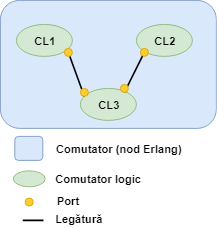
\includegraphics{linc_architecture}
	\caption{Arhitectura comutatorului software LINC \cite{linc2014qsg}.}
	\label{fig:linc_architecture}
\end{figure}

După cum este prezentat în \cite{linc2014qsg}, \gls{linc} prezintă mai multe blocuri software: comutatorul capabil OpenFlow, modului protocolului OpenFlow, modului protocolului OF-Config. Acestea sunt dezvoltate ca aplicații Erlang separate, respectând principiile \textit{Platforma Telecom Deschisă} - \gls{otp} ale limbajului Erlang. Există și o componentă separată care se ocupă de conexiunea la un echipament de control \gls{sdn}. Tabelele de fluxuri, porturile sau tabelele de grup sunt administrate de implementările separate reprezentând diferitele versiuni ale protocolului OpenFlow.

\subsubsection{LINC-OE}

Datorită naturii modulare a comutatorului \gls{linc}, a apărut o nouă implementare care să acopere cazurile de utilizare ale \gls{sdn} din domeniul optic: \gls{linc-oe}. Acesta reprezintă un simulator de comutatoare optice care suportă extensiile optice ale protocolului OpenFlow. Diferenţa dintre \gls{linc} și \gls{linc-oe} este că, în cazul celui din urmă, comutatoarele logice care sunt simulate reprezintă comutatoare optice, astfel că spre deosebire de interfeţele electrice, porturile optice oferă mai multe canale de comunicaţie independente, diferenţiate prin lungimea de undă. În implementarea \gls{linc-oe}, mesajele ce se transmit printr-un astfel de port optic nu mai sunt pachete Ethernet, ci mesaje Erlang, ce conţin informații adiţionale, pe lângă pachetul Ethernet propriu-zis. O altă diferenţă este dată de faptul ca \gls{linc-oe} oferă interfețe pentru simularea defectării legăturilor dintre porturi.

\subsubsection{Interfaţa NETCONF}

Comutatorul software \gls{linc} expune de asemenea și o interfață \gls{netconf}. Este folosită de către protocolul OF-Config și este disponibilă pentru un comutator doar dacă acel protocol este folosit. În cazul în care este permisă utilizarea acestuia, o nouă aplicație Erlang este pornită în cadrul nodului Erlang: \textit{enetconf}, care pornește un server \gls{netconf} ce așteaptă conexiuni pe IP-ul și portul selectate de utilizator.

Această abordare prezintă un dezavantaj major: un singur server \gls{netconf} este pornit pentru comutatorul \gls{linc}, astfel că nu se pot accesa comutatoarele logice care alcătuiesc comutatorul \gls{linc} individual prin interfața \gls{netconf}. Acestea pot fi configurate doar prin intermediul protocolului OpenFlow.

De asemenea, modelul informațional \gls{yang} care este expus de către server nu este configurabil, astfel încât utilizatorul nu poate alege un model \gls{yang} pe care comutatorul software să îl poată folosi. Dacă acest lucru ar fi fost oferit, ar fi fost banală transformarea \gls{linc-oe} în \gls{linc-we}, prin înlocuirea modelului \gls{yang} expus cu modelul informațional pentru microunde și apoi corelarea atributelor \gls{yang} cu parametrii comutatorului \gls{linc}.

\subsubsection{\textit{mininet}}

\subsection{LINC-WE}